\chapter{Grundlagen}
\label{chap:grundlagen}
Das Kapitel Grundlagen behandelt die Themen, die in mehreren Abschnitten dieser Arbeit relevant sind. Dabei handelt es sich um das Robot Operation System, die verwendeten Koordinatensysteme und die Transformation zwischen ihnen.

\section{Das Robot Operation System \gls{ros}}
\label{sec:ros}
Ziel dieses Unterkapitel ist es das Opensource Betriebssystem \gls{ros} vorzustellen. Wie es aufgebaut ist und welche Vorz�ge es besitzt.\\

\gls{ros} stellt dem Softwareentwickler Bibliotheken und Werkzeuge zur Verf�gung, die Helfen Roboteranwendungen zu erstellen. Das auf einem \gls{ip}-basierende  modulare Kommunikationsframework erm�glicht die Verkn�pfung von Anwendungssoftware, Sensoren und Aktoren sogar unter mehreren Robotern. Die Grundlage daf�r ist die sogenannte Hardwareabstraktion. Dabei wird durch hardwarespezifische Module erreicht, das Komponenten unterschiedlicher Hersteller miteinander verbunden werden k�nnen. In unserem Fall Hokuyo Lasersanner und \gls{asctec} \gls{fcu}. Au�erdem erm�glicht es eine hardwareunabh�ngige Programmierung, die  in den Programmiersprachen C/C++ oder in Python erfolgen kann. Jede Hardwareabstraktion oder Anwendung wird als Node, bzw. Konten bezeichnet und l�uft als eigener Prozess.
\begin{figure}
	\centering
	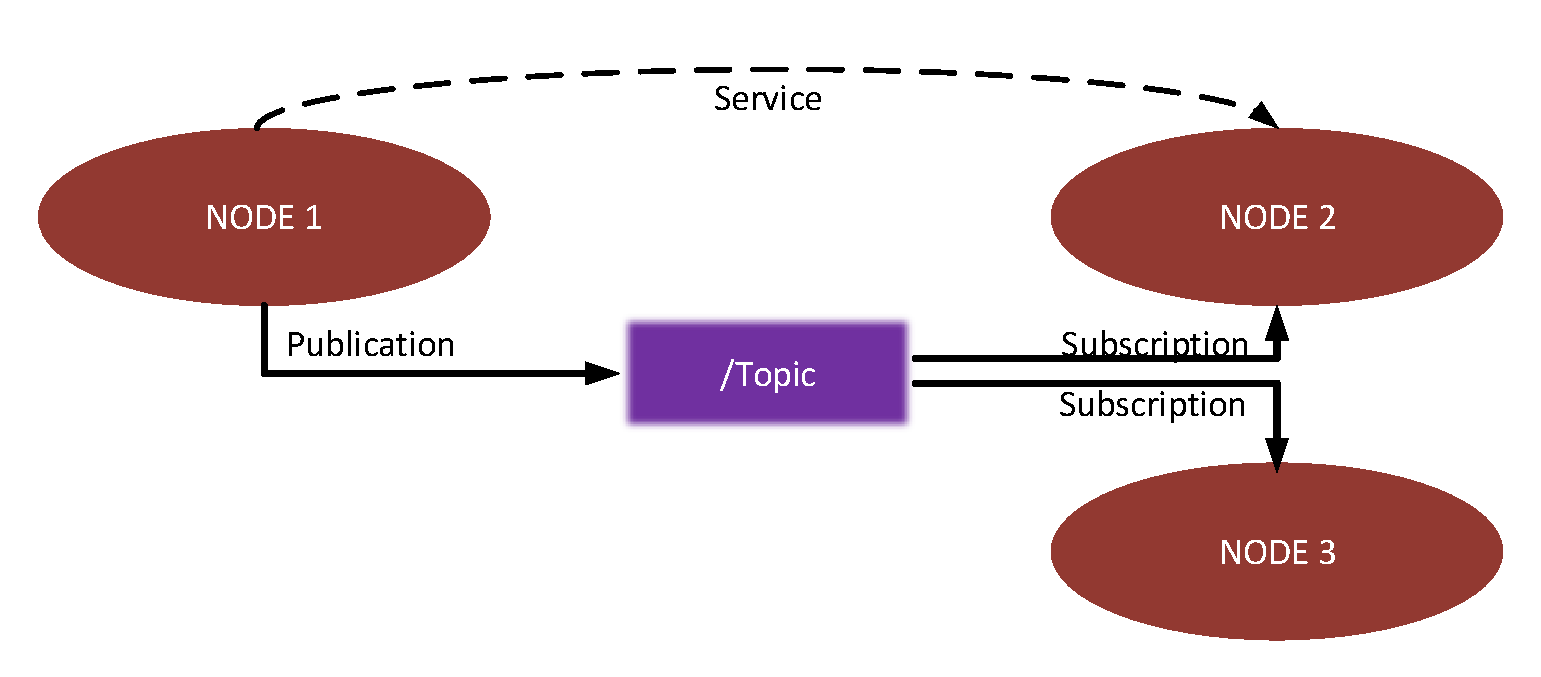
\includegraphics[width = 0.75\textwidth]{images/TopicUndService}
	\caption[Topic und Service]{Kommunikation von Nodes �ber Topics und Services}
	\label{fig:node_kommunikation}
\end{figure}


Der Austausch von Daten zwischen den Nodes erfolgt �ber so genannte Topics (Abbildung \ref{fig:node_kommunikation}]. Dabei werden von den Knoten Nachrichten (engl. Messages) in Topics gepostet und somit ver�ffentlicht (publication). Ben�tigt ein weiter Knoten den Inhalt dieses Topic kann er es abonnieren (subscription). Sobald die Nachricht im Knoten aktualisiert wurde, wird sie den abonnierenden Knoten �bertragen. Dabei sind Knoten nicht auf ein Topic beschr�nkt, es k�nnen beliebig viele Topics beschrieben oder empfangen werden. Alternative zu dieser Art der asynchronen Daten�bertragung, biete \gls{ros} die M�glichkeit einer Synchrone Kommunikation zwischen zwei Nodes �ber Services. Dabei wird auf einem Knoten ein Service gestartet. Dieser dient als Server und agiert nach dem Anfrage-Antwort-Prinzip. Schickt ein anderer Knoten eine Anfrage, wird ihm die geforderte Nachricht zu gesendet. 

Anzumerken ist, das durch das verwendete \gls{ip}-Protokoll keine deterministische Versendung der Nachrichten nicht gew�hrleistet ist, da es sein kann, das Nachrichten gleichen Types in Paketen zusammengefasst werden. Bei der Programmierung empfiehlt es sich daher auf Topics mit einem Zeitstempel (engl. timestamp) zur�ckzugreifen. Die Echtzeitf�higkeit des \gls{ros} ist durch allerdings nicht gef�hrdet. 

\begin{figure}
	\centering
	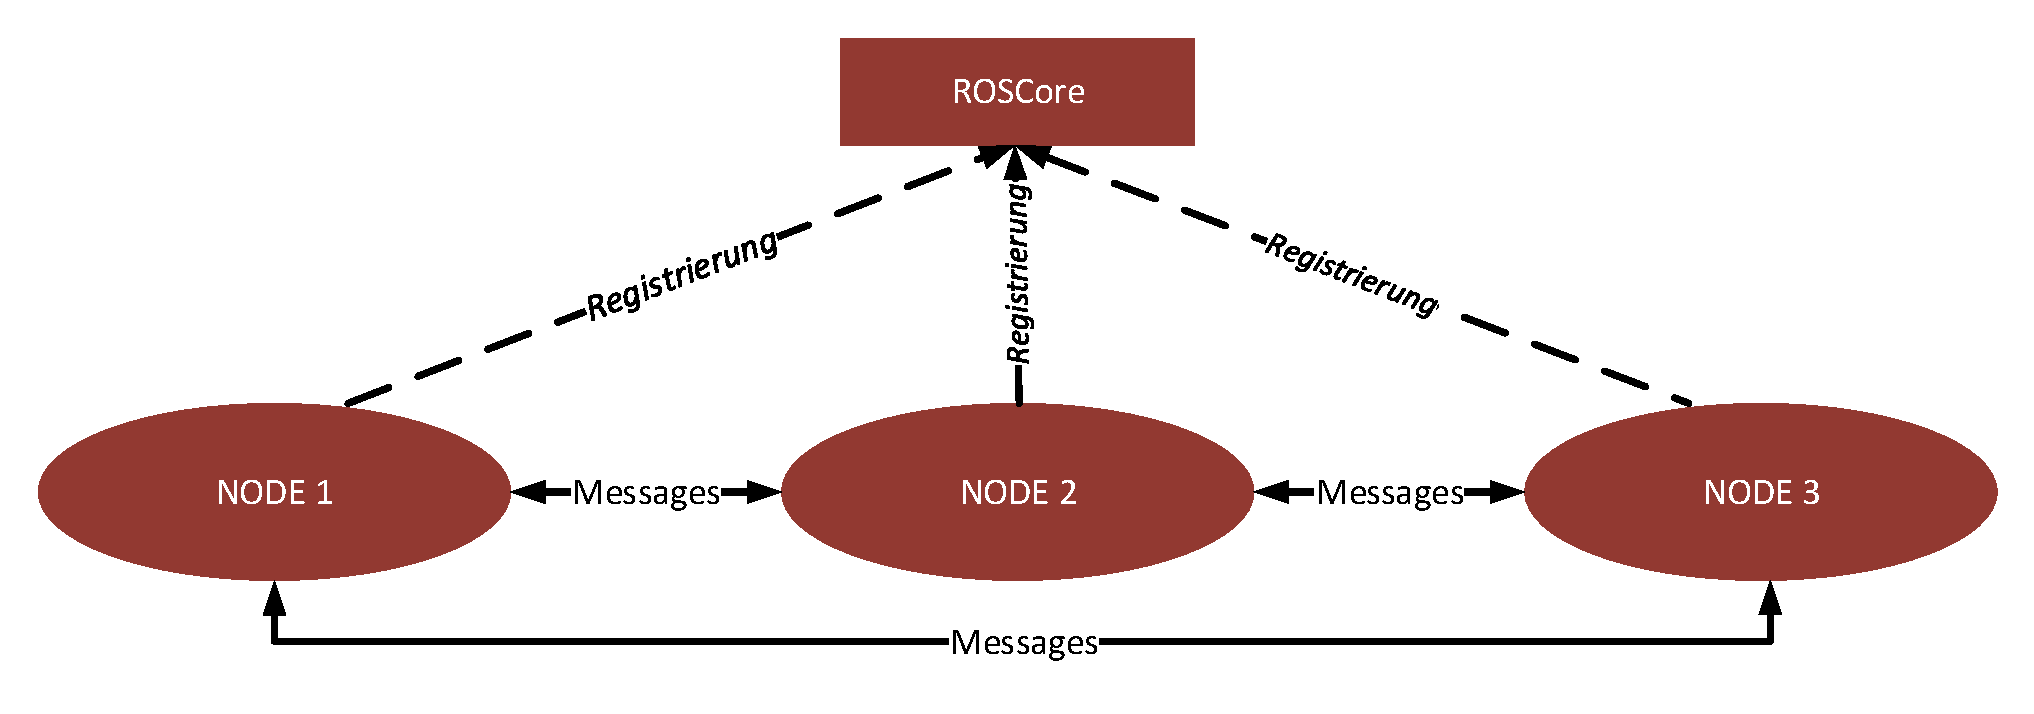
\includegraphics[width = \textwidth]{images/MasterAndNode}
	\caption[Registrierung der Knoten]{Registrierung der Knoten}
	\label{fig:node_master}
\end{figure}


Der wohl gr��te Vorteil von \gls{ros} ist die st�ndig wachsende Community. So stellen Forscher aus der ganze Welt ihre Algorithmen und Hardwareabstraktionen zur Verf�gung. Dadurch ist es m�glich bei der Erstellung einer Roboteranwendung auf Bausteine zur�ck zugreifen, die ohne diese Plattform selbst zu implementieren w�ren.


\section{Einf�hrung in die Koordinatensysteme und Koordinatentransformationen}
\label{sec:koordinatensysteme&transformationen}
Anhand von Koordinatensystemen und Transformationen l�sst sich die Lage eines Objektes in einen Raum mathematisch beschreiben. Die Grundvoraussetzung zur Bestimmung der Position des Quadrocopters im 2D-Raum (siehe Kapitel HIER MUSS NOCH EINE REFERENZ HIN). Au�erdem erm�glicht die Einf�hrung von Koordinatensystemen die mathematisch/physikalische Beschreibung des Quadrocopters und stellt somit die Grundlage zur Modellbildung und Reglerentwurf (siehe Kapitel so und so).  

\subsection{Koordinatensysteme}
\label{subsec:koordinatensysteme}
�ber ein Koordinatensystem l�sst sich die Position eines Punktes bezogen den Koordinatenursprung als Bezugspunkt, in einer zweidimensionalen Ebene, bzw in einem dreidimensionalen Raum �ber einen Vektor beschreiben.  


Es ist drauf hinzuweisen, dass es zur Navigation auf dem Erdball rotationsellipsische Koordinatensysteme ben�tigt werden [THIELECKE]. Diese Kr�mmung kann bei 

Bei der Indoornavigation kann die Kr�mmung der Erde vernachl�ssigt werden.
\begin{figure}
	
	\centering{
		\subfloat[ENU-Koordinatensystem]{
			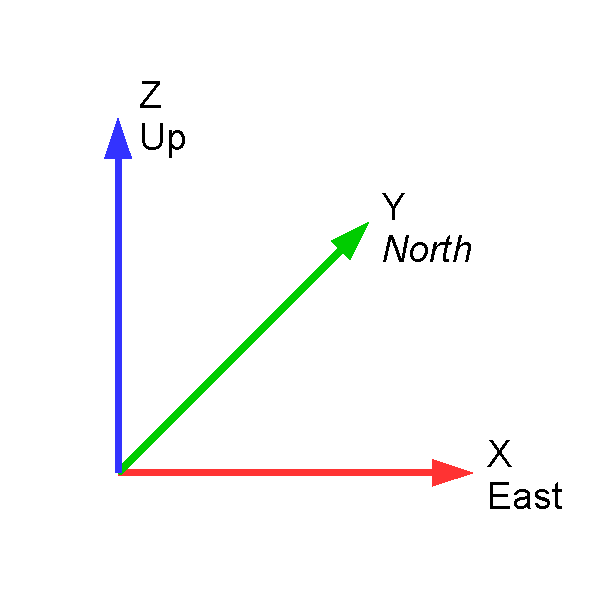
\includegraphics[width=0.3\textwidth]{images/ENU-koordinatensystem}
			\label{fig:enu}
		}
		\subfloat[NED-Koordimatemsystem]{
			\includegraphics[width=0.3\textwidth]{images/ned-koordinatensystem}
			\label{fig:ned}
		}
	}
	\caption[Kovention ]{test}

\end{figure}


 \begin{figure}
 	\centering
 	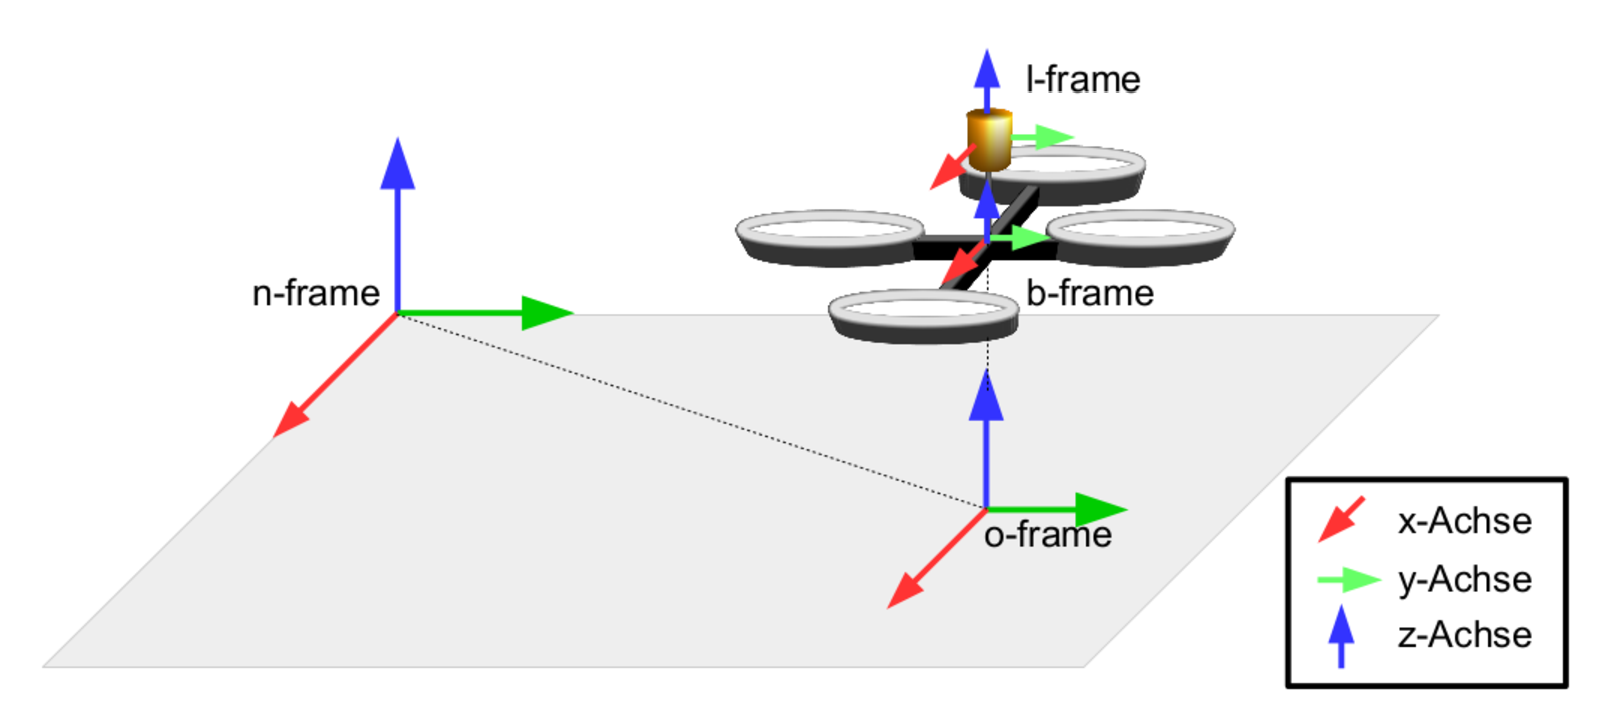
\includegraphics[width = \textwidth]{images/Koordinatensysteme}
 	\caption[Koordinatensysteme]{In der Arbeit angewandte Koordinatensysteme }
 	\label{fig:koordinatensysteme}
 \end{figure}
\subsection{Koordinatentransformationen}
\label{subsec:koordinatentransformation}


